\documentclass[dvipsnames]{beamer}
\usepackage{comment}
\usepackage{hyperref}
\usepackage{graphicx}

\title{MATH 1190 \& 1210 Meeting for Week 14}
\author{Josh}
\date{13 April 2026}

\newcommand{\transition}[1]{\frame{{}\begin{center}\fbox{#1}\end{center}}}

\begin{document}

\maketitle


\section{Logistics: Pacing}

\transition{Logistics}

\frame{{Logistics: Pacing}

{\bf Where are folks in the lessons right now?}

}



\section{Logistics: Application Day 3}

\transition{Logistics}

\frame{{Logistics: Application Day 3}

{\bf How did the Gradient Descent Application go?}

}
\frame[t]{{Logistics: Upcoming Schedule}

    \begin{itemize}
       \item week 14 of class (13 April - 17 April)
        \begin{itemize}
        \item lesson 21 (Continuous RVs)
        \item lesson 22 (Expectation and Variance) -- {\footnotesize\color{red} last topic on assessment 4}
        \end{itemize}
    \item week 15 of class (20 April - 24 April)
        \begin{itemize}
        \item Application Day 4: Markov Chains
        \item Review + catch up (if needed)
        \item KC 4 on Thursday 23 April 
        \end{itemize}
     \item week 16 of class (27 April - 1 May)
            \begin{itemize}
        \item Review
        \item Final Exam on Friday 1 May
        \end{itemize}

    \end{itemize}

}

\frame[t]{{Logistics: Upcoming Deadlines}

{\bf Assessment-related Logistics}
\begin{itemize}
\item KC3 Reflections: Due Tuesday 14 April
\item KC3 Regrade requests open now due by Thursday 16 April
\item KC4 next week 23 April
    \begin{itemize}
    \item reassessment targets: {\color{RedOrange}A2},{\color{RedOrange}A3}, {\color{Fuchsia}I1}, {\color{Fuchsia}I2}, 
    \item new targets:{\color{Fuchsia}I3},{\color{Fuchsia}I4},{\color{ProcessBlue}F3}, {\color{Orange}P1}, {\color{Orange}P2} (5 targets!)
    \item Thursday, 23 April, 7:00 PM; 80 minutes
    \item Room assignments same as KC1 this time. No switching dates!
    \end{itemize}
\end{itemize}

}

\frame[t]{{Logistics: D2 D3 Mixup}

{\bf Assessment-related Logistics}
\begin{itemize}
\item Labels will be switched and any student that earned proficiency on the correct target will still receive profiiency
\item Filtered KC2 and KC3 for students that earned proficiency on either D2 or D3 but not both.
\item Found all students that had proficiency on either D2 on KC2 and "D3" on KC3 and same for D3
\item Six students could be affected by the mixup
\end{itemize}

}
\begin{frame}{D2 D3 Mixup}
\begin{center}
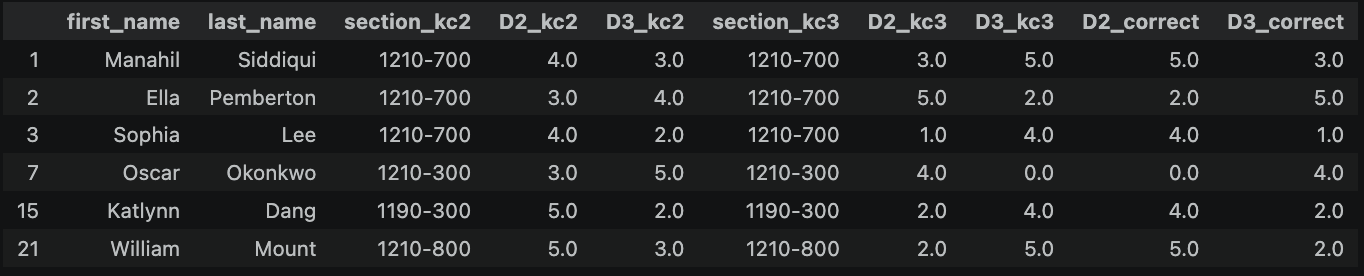
\includegraphics[width=\textwidth]{KCMixup.png}
\end{center}
\end{frame}
\frame{{Logistics: LA Performance}

{\bf How has everyone's LA been this semester?}

}


\section{Content}

\transition{Content}


%------------------------------------------------

%------------------------------------------------

%------------------------------------------------

\begin{frame}{Learning Goals}
\begin{itemize}
    \item Distinguish between discrete and continuous random variables
    \item Understand probability density functions (PDFs)
    \item Define and identify support
    \item Compute probabilities using integrals
    \item Understand and compute cumulative distribution functions (CDFs)
\end{itemize}
\end{frame}

%------------------------------------------------

\begin{frame}{Warm-Up: Discrete vs Continuous}
\textbf{Key Idea:} What kind of values can the variable take?

\begin{itemize}
    \item Discrete: counts (e.g., number of arrivals, number of children)
    \item Continuous: measurements (e.g., temperature, time)
\end{itemize}

\textbf{Takeaway:}
\begin{itemize}
    \item Discrete $\rightarrow$ countable values
    \item Continuous $\rightarrow$ any value in an interval
\end{itemize}
\end{frame}

%------------------------------------------------

\begin{frame}{Motivation: From Histograms to Density}
\begin{itemize}
    \item Histograms approximate distributions
    \item For continuous data, we “smooth” into a curve
\end{itemize}

\textbf{Key Concept: Probability Density Function (PDF)}
\begin{itemize}
    \item Area under curve = probability
    \item Total area = 1
\end{itemize}
\end{frame}

%------------------------------------------------

\begin{frame}{Probability Density Function (PDF)}
\textbf{Definition:}
\[
P(a < X < b) = \int_a^b p(x)\,dx
\]

\textbf{Properties:}
\begin{itemize}
    \item $p(x) \ge 0$
    \item Total area = 1
\end{itemize}

\textbf{Support:}
\begin{itemize}
    \item Interval where $p(x) > 0$
\end{itemize}
\end{frame}

%------------------------------------------------

\begin{frame}{Example: Waiting for a Bus (Uniform)}
\textbf{Setup:}
\begin{itemize}
    \item Wait time between 0 and 30 minutes
    \item All times equally likely
\end{itemize}

\textbf{Key Ideas:}
\begin{itemize}
    \item Support: $[0,30]$
    \item PDF is constant (uniform)
    \item Probability = area = rectangle
\end{itemize}
\end{frame}

%------------------------------------------------

\begin{frame}{Using the PDF}
\textbf{Main Skill:}
\begin{itemize}
    \item Compute probabilities using integrals
\end{itemize}

\textbf{Example Flow:}
\begin{itemize}
    \item Find constant using total area = 1
    \item Integrate over interval to find probability
    \item Solve for unknown bounds if needed
\end{itemize}
\end{frame}

%------------------------------------------------

\begin{frame}{Practice: Building a PDF}
\textbf{Key Steps:}
\begin{enumerate}
    \item Identify support
    \item Use $\int p(x)dx = 1$ to find constants
    \item Compute probabilities with integrals
\end{enumerate}

\textbf{Big Idea:}
PDFs must be valid probability models (area = 1)
\end{frame}

%------------------------------------------------

\begin{frame}{Cumulative Distribution Function (CDF)}
\textbf{Definition:}
\[
C(x) = P(X \le x) = \int_a^x p(t)\,dt
\]

\textbf{Interpretation:}
\begin{itemize}
    \item Measures accumulated probability
\end{itemize}

\textbf{Connection:}
\[
p(x) = C'(x)
\]
\end{frame}

%------------------------------------------------

\begin{frame}{Properties of the CDF}
\begin{itemize}
    \item Always increasing
    \item Starts at 0, ends at 1
    \item Never decreases
\end{itemize}

\textbf{Probability from CDF:}
\[
P(c \le X \le d) = C(d) - C(c)
\]
\end{frame}

%------------------------------------------------

\begin{frame}{Example: Uniform CDF}
\textbf{Key Ideas:}
\begin{itemize}
    \item Integrate PDF to get CDF
    \item Piecewise function:
    \begin{itemize}
        \item 0 before support
        \item Increasing within support
        \item 1 after support
    \end{itemize}
\end{itemize}
\end{frame}

%------------------------------------------------

\begin{frame}{Working with the CDF}
\textbf{Skills Developed:}
\begin{itemize}
    \item Find CDF from PDF
    \item Interpret graphs
    \item Find median using $C(x)$
\end{itemize}

\textbf{Median Idea:}
\[
P(X < m) = 0.5
\]
\end{frame}

%------------------------------------------------

\begin{frame}{Graph Interpretation}
\textbf{Key Questions:}
\begin{itemize}
    \item Is it a PDF or CDF?
    \item What is the support?
    \item How to compute probabilities?
\end{itemize}

\textbf{Clues:}
\begin{itemize}
    \item CDF: increasing, ends at 1
    \item PDF: area = probability
\end{itemize}
\end{frame}

%------------------------------------------------

\begin{frame}{From CDF to PDF}
\textbf{Key Idea:}
\begin{itemize}
    \item PDF is the slope (derivative) of CDF
\end{itemize}

\textbf{Interpretation:}
\begin{itemize}
    \item Steeper slope $\rightarrow$ higher density
\end{itemize}
\end{frame}

%------------------------------------------------

\begin{frame}{Lesson Summary}
\begin{itemize}
    \item Continuous variables use PDFs instead of probabilities at points
    \item Probabilities = area under curve
    \item CDF accumulates probability
    \item PDF and CDF are linked by derivatives/integrals
    \item Graphs help interpret distributions
\end{itemize}
\end{frame}

%------------------------------------------------
%%%%%%%%%%%%%%%%%%%%%%%%%%%%%%%%%%%%%%%%%%%%%%%%%%%%%%%%%%%%%%%%%%%%%%%%%%%%%%%%%%%%%%%%%%%%%%%%%%%%%%
%%%%%%%%%%%%%%%%%%%%%%%%%%%%%%%%%%%%%%%%%%%%%%%%%%%%%%%%%%%%%%%%%%%%%%%%%%%%%%%%%%%%%%%%%%%%%%%%%%%%%%


%------------------------------------------------

\begin{frame}{Learning Goals}
\begin{itemize}
    \item Understand expectation (mean) and variance
    \item Compute expectation and variance for discrete variables
    \item Compute expectation and variance for continuous variables
    \item Interpret spread and variability
\end{itemize}
\end{frame}

%------------------------------------------------

\begin{frame}{Motivation}
\textbf{Two Key Questions:}
\begin{itemize}
    \item Where is the distribution centered? (Mean)
    \item How spread out is it? (Variance)
\end{itemize}

\textbf{Key Ideas:}
\begin{itemize}
    \item Expectation = long-run average
    \item Variance = variability around the mean
\end{itemize}
\end{frame}

%------------------------------------------------

\begin{frame}{Discrete Expectation and Variance}
\textbf{Formulas:}
\[
E[X] = \sum x\,p(x)
\]
\[
Var(X) = E[X^2] - (E[X])^2
\]

\textbf{Key Idea:}
\begin{itemize}
    \item Weighted average using probabilities
\end{itemize}
\end{frame}

%------------------------------------------------

\begin{frame}{Example: Sum of Coin Flips}
\textbf{Setup:}
\begin{itemize}
    \item Flip a coin 3 times
    \item Random variable = total number of 1s
\end{itemize}

\textbf{Main Ideas:}
\begin{itemize}
    \item Compute mean as weighted average
    \item Compute variance using $E[X^2] - \mu^2$
\end{itemize}

\textbf{Takeaway:}
\begin{itemize}
    \item Expectation gives center of distribution
\end{itemize}
\end{frame}

%------------------------------------------------

\begin{frame}{Understanding Variance (Graphs)}
\textbf{Key Idea: Spread Matters}

\begin{itemize}
    \item Same mean, different spreads $\rightarrow$ different variances
    \item More mass at extremes $\rightarrow$ higher variance
    \item More mass near center $\rightarrow$ lower variance
\end{itemize}
\end{frame}

%------------------------------------------------

\begin{frame}{Comparing Distributions}
\textbf{Visual Reasoning:}
\begin{itemize}
    \item Narrow distribution $\rightarrow$ small variance
    \item Wide distribution $\rightarrow$ large variance
\end{itemize}

\textbf{Skill:}
\begin{itemize}
    \item Rank variance without calculations
\end{itemize}
\end{frame}

%------------------------------------------------

\begin{frame}{Designing Distributions}
\textbf{Key Ideas:}
\begin{itemize}
    \item Increase variance: move probability to extremes
    \item Decrease variance: concentrate near mean
\end{itemize}

\textbf{Insight:}
\begin{itemize}
    \item Variance measures spread, not location
\end{itemize}
\end{frame}

%------------------------------------------------

\begin{frame}{Continuous Expectation and Variance}
\textbf{Formulas:}
\[
E[X] = \int x\,p(x)\,dx
\]
\[
Var(X) = \int x^2 p(x)\,dx - (E[X])^2
\]

\textbf{Key Idea:}
\begin{itemize}
    \item Continuous version of weighted average
\end{itemize}
\end{frame}

%------------------------------------------------

\begin{frame}{Example: Continuous Distribution}
\textbf{Main Steps:}
\begin{itemize}
    \item Multiply by $x$ (or $x^2$)
    \item Integrate over support
    \item Subtract $\mu^2$ for variance
\end{itemize}

\textbf{Takeaway:}
\begin{itemize}
    \item Same process as discrete, but with integrals
\end{itemize}
\end{frame}

%------------------------------------------------

\begin{frame}{Finding a PDF from Information}
\textbf{Key Skills:}
\begin{itemize}
    \item Identify PDF from expectation expression
    \item Use total probability = 1 to find constants
\end{itemize}

\textbf{Important Rule:}
\[
\int p(x)\,dx = 1
\]
\end{frame}

%------------------------------------------------

\begin{frame}{Computing Variance (Continuous)}
\textbf{Steps:}
\begin{enumerate}
    \item Compute $E[X]$
    \item Compute $E[X^2]$
    \item Use $Var(X) = E[X^2] - (E[X])^2$
\end{enumerate}

\textbf{Common Pitfall:}
\begin{itemize}
    \item Forgetting to square the mean
\end{itemize}
\end{frame}

%------------------------------------------------

\begin{frame}{Discrete Practice Ideas}
\textbf{Skills:}
\begin{itemize}
    \item Complete a PMF (probabilities sum to 1)
    \item Compute expectation
    \item Compute variance
\end{itemize}

\textbf{Big Idea:}
\begin{itemize}
    \item Everything comes from weighted sums
\end{itemize}
\end{frame}

%------------------------------------------------

\begin{frame}{Continuous Practice Ideas}
\textbf{Skills:}
\begin{itemize}
    \item Set up integrals correctly
    \item Handle powers of $x$
    \item Work with logarithmic PDFs
\end{itemize}

\textbf{Insight:}
\begin{itemize}
    \item Structure matters more than computation
\end{itemize}
\end{frame}

%------------------------------------------------

\begin{frame}{Lesson Summary}
\begin{itemize}
    \item Expectation = center (average outcome)
    \item Variance = spread around the mean
    \item Discrete $\rightarrow$ sums
    \item Continuous $\rightarrow$ integrals
    \item Graphs help interpret variance visually
\end{itemize}
\end{frame}

%------------------------------------------------

%%%%%%%%%%%%%%%%%%%%%%%%%%%%%%%%%%%%%%%%%%%%%%%%%%%%%%%%%%%%%%%%%%%%%%%%%%%%%%%%%%%%%%%%%%%%%%%%%%%%%%
%%%%%%%%%%%%%%%%%%%%%%%%%%%%%%%%%%%%%%%%%%%%%%%%%%%%%%%%%%%%%%%%%%%%%%%%%%%%%%%%%%%%%%%%%%%%%%%%%%%%%%

\section{Pedagogy}

\transition{Pedagogy}


\transition{Active Learning}
\transition{And Now - An Active Learning Discussion with Vadim!}
%%%%%%%%%%%%%%%%%%%%%%%%%%%%%%%%%%%%%%%%%%%%%%%%%%%%%%%%%%%%%%%%%%%%%%%%%%%%%%%%%%%%%%%%%%%%%%%%%%%%%%

%------------------------------------------------

%------------------------------------------------

\begin{frame}{Purpose of the Paper}
\href{https://www.frontiersin.org/journals/education/articles/10.3389/feduc.2024.1388720/full}{\bf ``Teaching dynamics to enhance critical thinking and knowledge socialization in the mathematics classroom"}
\begin{itemize}
    \item Investigates how teaching practices influence critical thinking in mathematics
    \item Moves beyond procedural fluency toward deep conceptual reasoning
    \item Emphasizes \textbf{classroom dynamics} rather than just curriculum design
\end{itemize}

\vspace{0.5cm}

\textbf{Core Claim:}
\begin{itemize}
    \item Critical thinking emerges from \textbf{how students engage}, not just what content is covered
\end{itemize}
\end{frame}

%------------------------------------------------

\begin{frame}{Defining “Critical Thinking” in Math?}
\begin{itemize}
    \item Interpreting and evaluating mathematical arguments
    \item Making connections across concepts
    \item Justifying reasoning and questioning assumptions
    \item Moving beyond computation to mathematical sense-making
\end{itemize}

\vspace{0.5cm}

\begin{itemize}
    \item From “getting answers” $\rightarrow$ explaining why and how
\end{itemize}
\end{frame}

%------------------------------------------------

\begin{frame}{Limitations}
\begin{itemize}
    \item Lecture-dominated environments
    \item Emphasis on procedures and correct answers
    \item Limited opportunities for student explanation or dialogue
\end{itemize}

\vspace{0.5cm}

\textbf{Result:}
\begin{itemize}
    \item Students may succeed computationally but lack transferable understanding
\end{itemize}
\end{frame}

%------------------------------------------------

\begin{frame}{Key Teaching Dynamics Identified}
\textbf{The paper highlights three core dynamics:}

\begin{itemize}
    \item \textbf{Knowledge Socialization}
    \begin{itemize}
        \item Students articulate and negotiate meaning
    \end{itemize}
    
    \item \textbf{Dialogic Interaction}
    \begin{itemize}
        \item Classroom discourse as a learning mechanism
    \end{itemize}
    
    \item \textbf{Student Agency}
    \begin{itemize}
        \item Students take ownership of reasoning processes
    \end{itemize}
\end{itemize}
\end{frame}

%------------------------------------------------

\begin{frame}{Knowledge Socialization}
\begin{itemize}
    \item Learning occurs through shared construction of ideas
    \item Students explain, challenge, and refine each other's thinking
\end{itemize}

\vspace{0.5cm}

\textbf{Instructor Role:}
\begin{itemize}
    \item Facilitate rather than transmit knowledge
\end{itemize}

\vspace{0.5cm}

\textbf{Implication:}
\begin{itemize}
    \item Understanding becomes collective, not individual
\end{itemize}
\end{frame}

%------------------------------------------------

\begin{frame}{Dialogic Interaction}
\begin{itemize}
    \item Emphasis and normalization of discussion-based learning
    \item Questions that drive exploration rather than confirm answers
\end{itemize}

\vspace{0.5cm}

\textbf{Key Idea:}
\begin{itemize}
    \item Quality of questions $\rightarrow$ depth of thinking
\end{itemize}

\vspace{0.5cm}

\textbf{Contrast:}
\begin{itemize}
    \item Traditional: teacher asks $\rightarrow$ student answers
    \item Dialogic: students question, respond, and build on ideas
\end{itemize}
\end{frame}

%------------------------------------------------

\begin{frame}{Student Agency}
\begin{itemize}
    \item Students actively construct and defend ideas
    \item Less reliance on instructor validation
\end{itemize}

\vspace{0.5cm}

\textbf{Indicators of Agency:}
\begin{itemize}
    \item Students initiate strategies
    \item Students critique reasoning (their own and others)
\end{itemize}

\vspace{0.5cm}

\textbf{Outcome:}
\begin{itemize}
    \item Deeper engagement and ownership of learning
\end{itemize}
\end{frame}

%------------------------------------------------

\begin{frame}{Implications for College Math Teaching}
\begin{itemize}
    \item Incorporate structured discussion into lectures
    \item Design tasks that require explanation, not just answers
    \item Encourage multiple solution paths
\end{itemize}

\vspace{0.5cm}

\textbf{How do we make the key shift:}
\begin{itemize}
    \item From content delivery $\rightarrow$ thinking development
\end{itemize}
\end{frame}

%------------------------------------------------

\begin{frame}{Tensions and Challenges}
\begin{itemize}
    \item Time constraints in content-heavy courses
    \item Large class sizes
    \item Student resistance to non-traditional formats
    \item Assessment misalignment (procedural exams vs conceptual goals)
\end{itemize}

\vspace{0.5cm}

\textbf{Core Tension:}
\begin{itemize}
    \item Coverage vs depth
\end{itemize}
\end{frame}

%------------------------------------------------

\begin{frame}{Discussion: Critical Thinking in Practice}

\begin{itemize}
    \item Where in our courses do students actually \textbf{reason} vs execute what we are showing them?
    \item Is this a reasonable expectation for students that struggle with core material?
    \item What proportion of class time do you typically spend on student thinking vs instructor explanation?
\end{itemize}
\end{frame}

%------------------------------------------------

\begin{frame}{Discussion: Classroom Dynamics}
\begin{itemize}
    \item How do we know when “productive mathematical discussion” is happening in our classrooms?
    \item How do we intervene without shutting down student reasoning?
    \item What norms are required for students to critique each other constructively?
\end{itemize}
\end{frame}
%------------------------------------------------
\begin{frame}{Key Teaching Dynamics Identified}
\textbf{How do we incorporate the three core dynamics into our own classrooms? Any ideas?}

\begin{itemize}
    \textbf{Knowledge Socialization}
    \begin{itemize}
        \item Students articulate and negotiate meaning
    \end{itemize}
    
    \item \textbf{Dialogic Interaction}
    \begin{itemize}
        \item Classroom discourse as a learning mechanism
    \end{itemize}
    
    \item \textbf{Student Agency}
    \begin{itemize}
        \item Students take ownership of reasoning processes
    \end{itemize}
\end{itemize}
\end{frame}
%------------------------------------------------

\begin{frame}{Discussion: Barriers}
\begin{itemize}
    \item What structural constraints do you feel limit these approaches?
    \item Which of these constraints are real vs perceived?
\end{itemize}
\end{frame}



%------------------------------------------------

\begin{frame}{Discussion: Implementation}
\begin{itemize}
    \item What is one small change that could increase student agency in our courses?
    \item What would you be willing to remove, if anything, to make space for deeper thinking?
\end{itemize}
\end{frame}

%------------------------------------------------

\begin{frame}{Takeaways}
\begin{itemize}
    \item Critical thinking is shaped by classroom interaction, not just content
    \item Discussion, explanation, and student agency are central
    \item How do teaching decisions influence how students experience mathematics?
\end{itemize}
\end{frame}

%------------------------------------------------



%------------------------------------------------

\end{document}


